\section{Zielsetzung}

In diesem Versuch soll die Wellenlänge eines Lasers und die Brechungsindizes von Luft bei verschiedenen Drücken mit einem Michelson-Interferometer untersucht werden.

\section{Theorie}
\label{sec:Theorie}

\subsection{Interferenzerscheinungen bei Licht}

Licht ist eine elektromagnetische Welle, bei der sich die Feldstärke am Ort $x$ und zum Zeitpunkt $t$ mittels der Maxwell-Gleichungen über

\begin{equation}
    \label{eqn:allg-loesung}
    E(x,t) = E_0 \cos(kx - \omega t - \delta)
\end{equation}

bestimmen lässt. Dabei ist $k = \dfrac{2\pi}{\lambda}$ mit der Wellenlänge $\lambda$ die Wellenzahl, $\omega$ die Kreisfrequenz und $\delta$ eine beliebige Phase.
Da die Maxwell-Gleichungen lineare partielle Differentialgleichungen sind, gilt für die Lösungen dieser, also in diesem Fall Gleichung \eqref{eqn:allg-loesung}, das Superpositionsprinzip.
In der Praxis wird häufig die Intensität gemessen, da diese sich einfacher beobachten lässt. Diese berechnet sich dabei über

\begin{equation}
    \label{eqn:intensitaet}
    I = \text{const} \cdot |E_0|^2.
\end{equation}

Damit ergibt sich bei der Superposition von zwei Wellen eine Intensität von

\begin{equation}
    I_\text{ges} = \text{const} \cdot 2 |E_0|^2 (1 + cos(\delta_2 - \delta_1)).
\end{equation}

Der letzte Summand bildet den sogenannten Interferenzterm. Dieser ist abhängig von den Phasen der beiden Wellen und sorgt dafür, dass die Gesamtintensität zwischen $+ \text{const} \cdot 2 |E_0|^2$ und $- \text{const} \cdot 2 |E_0|^2$ schwanken kann.
Daraus folgt des Weiteren, dass die Intensität verschwindet, wenn $\delta_2 - \delta_1$ ein ungerades Vielfaches von $\pi$ ist.

Es ist jedoch zu beachten, dass Licht aus verschiedenen Quellen im Allgemeinen nicht interferenzfähig ist.
Dies liegt daran, dass das Licht bei der Emittierung in Atom statistisch verteilt ist und der Interferenzterm verschwindet, wenn über einen genügend großen Zeitraum gemittelt wird.
Diese Art von Licht wird inkohärent genannt. Im Gegensatz dazu steht das sogenannte kohärente Licht, welches nach Gleichung \eqref{eqn:allg-loesung} ein festes $k$, $\omega$ sowie $\delta$ besitzt.
In der Praxis werden häufig Laser genutzt, um solches Licht zu erzeugen.
Dabei ist die sogenannte Kohärenzlänge $l_C$ eben diese, die das Licht in der Zeit zurücklegt, in der von der Quelle noch Licht mit den oben benannten Eigenschaften aussendet.
Bei natürlichem Licht liegt dies im Bereich von $10^{-6}$ m, Laser hingegen erreichen weit höhere Längen.

\subsection{Das Michselson-Interferometer}

Bei dem Michselson-Interferometer wird ein Lichtstrahl mit einem semipermeablen Material wie in \autoref{fig:michelson} geteilt.

\begin{figure}
    \centering
    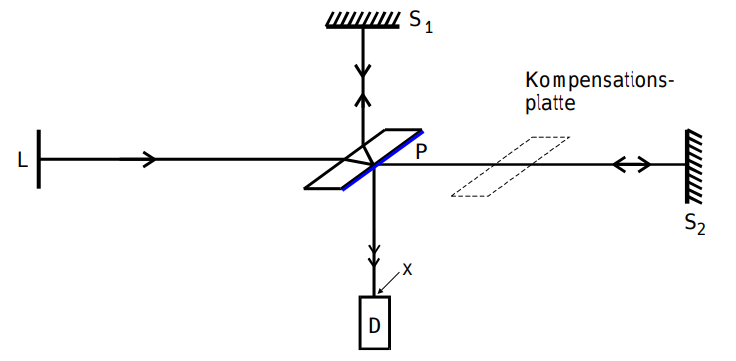
\includegraphics[width=0.9\textwidth]{content/michelson.png}
    \caption{Aufbau eines Michelson-Interferometers \cite{V401}.}
    \label{fig:michelson}
\end{figure}

Dabei läuft ein Teil des Lichtes durch durch das Material und wird an dem Spiegel $S_2$ reflektiert, ein anderer Teil wird an dem Material selbst reflektiert und läuft zu Spiegel $S_1$.
Beide Strahlen sollen senkrecht auf die Spiegel auftreffen, sodass sie in umgekehrte Einfallsrichtung reflektiert werden und sich im semipermeablen Material überlagern. Zu bemerken ist, dass an dieser Stelle wieder Strahlteilungen existieren, jedoch wird im Weiteren nur noch der Strahl zum Detektor betrachet.
Dieser nimmt Intensitätsminima und -maxima auf und kann so Interferenzerscheinungen messen.
Wichtig ist dabei, dass die Strahlen kohärent sein müssen, weshalb die Abstände $\overline{S_1P}$ und $\overline{S_2P}$ nahezu gleich sein müssen.
Des Weiteren wird zwischen $P$ und $S_2$ eine Kompensationsplatte angebracht, da dieser Strahl nicht durch das semipermeable Material laufen und die optische Weglänge ansonsten unterschiedlich wäre.

Verschiebt man den einen der Spiegel um eine Distanz $\Delta d$ so ergibt sich für die Anzahl der Intensitätsmaxima der Zusammenhang

\begin{equation}
    \label{eqn:verschieben}
    \Delta d = \frac{z \lambda}{2}.
\end{equation}

Des Weiteren kann ein optischer Wegunterschied erzeugt werden in dem vor einem der Spiegel ein Medium der Breite $b$ und mit dem Brechungsindex $n + \Delta n$ angebracht wird.
Dann lässt sich der oben beschriebenen Zusammenhang als

\begin{equation}
    \label{eqn:brech}
    b \Delta n = \frac{z \lambda}{2}
\end{equation}

schreiben.
Praktisch lässt sich das $\Delta n$ durch Druckänderung in einem Gas realisieren. Generell gilt für den Brechungsindex

\begin{equation}
    n = \sqrt{1 + f(\lambda) N},
\end{equation}

wobei $N$ die Zahl der zu Schwingungen angeregten Dipole pro Volumeneinheit ist. Jedoch ist im Bereich des sichtbaren Lichtes $fN \ll 1$ weshalb die Näherung

\begin{equation}
    n = 1 + \frac{fN}{2}
\end{equation}

genutzt werden kann. Bei Drücken zwischen 0 und 1 bar kann des Weiteren angenommen werden, dass Gase sich wie ideale Gase verhalten.
Daraus folgt der Zusammenhang

\begin{equation}
    N(p, T) = \frac{pT_0}{Tp_0}N_L,
\end{equation}

wobei $N_L$ die Loschmidtsche Zahl ist und $T_0$ sowie $p_0$ Normalbedingungen beschreiben.
Damit lässt sich der Zusammenhang

\begin{equation}
    \label{eqn:delta-n}
    \Delta n (p, p') = \frac{f}{2} N_L \frac{T_0}{p_0} \frac{1}{T}(p-p')
\end{equation}

finden. Damit lässt sich den Brechungsindex unter Normalbedingungen als

\begin{equation}
    \label{eqn:n-final}
    n (p_0, T_0) = 1 + \Delta n(p, p') \frac{T}{T_0}\frac{p_0}{p-p'}
\end{equation}

schreiben.